\documentclass[t,aspectratio=169]{beamer} % 使用16:9宽高比
\usetheme{Madrid} % 选择Madrid主题
\usecolortheme{default} % 使用默认颜色主题

% 设置字体
\usepackage[UTF8]{ctex}
\usefonttheme{structurebold} % 加粗结构字体

% 数学包
\usepackage{amsmath, amssymb, bm}
\usepackage{url}
\usepackage{booktabs}

% 图形包
\usepackage{graphicx}

% 标题页信息
\title[9.5.残差连接]{第9章：正则化}
\subtitle{第5节：残差连接 (Residual Connections)}
\author{《深度学习基础》课程小组}
% \institute{上海立信会计金融学院}
\date{\today}

\begin{document}

% 标题页
\frame{\titlepage}

% 目录页
\begin{frame}
    \frametitle{目录}
    \tableofcontents
\end{frame}

% ============================================================
% 第一部分：深度网络的挑战
% ============================================================
\section{深度网络的挑战}

\begin{frame}
    \frametitle{1. 深度网络的训练困难}
    \begin{itemize}
        \item 深度神经网络的表示能力很大程度上源于\alert{多层处理}。
        \item 增加层数可\alert{显著提升泛化性能}。
        \item 批归一化 + 仔细初始化可帮助解决\alert{梯度消失/爆炸}问题。
        \item \textbf{但即使有批归一化}，训练很多层的网络仍然越来越困难。
    \end{itemize}
\end{frame}

\begin{frame}
    \frametitle{1.1 破碎梯度 (Shattered Gradients)}
    \begin{itemize}
        \item 对这一现象的一种解释：\alert{破碎梯度}。
        \item 神经网络的表示能力随深度\alert{指数级增长}。
        \item ReLU 激活函数：网络可表示的\alert{线性区域数量指数级增长}。
        \item \textbf{后果}：误差函数梯度中的\alert{不连续性激增}。
        \item 图 9.12：输出对输入的导数（雅可比）作为输入的函数。
        \item 由链式法则，这些导数决定了误差函数曲面的梯度。
        \item \textbf{观察}：
        \begin{itemize}
            \item 深层网络中，早期层权重的\alert{极小变化}可导致梯度的\alert{显著变化}。
            \item 基于梯度的迭代优化假设梯度在参数空间中\alert{平滑变化}。
            \item 破碎梯度效应使极深网络的训练\alert{失效}。
        \end{itemize}
    \end{itemize}
\end{frame}

% ============================================================
% 第二部分：残差连接
% ============================================================
\section{残差连接}

\begin{frame}
    \frametitle{2. 残差连接 (Residual Connections)}
    \begin{itemize}
        \item 对网络架构的重要修改，极大帮助训练极深网络（He et al., 2015）。
        \item 是\alert{跳跃层连接}（skip-layer connections）的一种特殊形式。
        \item 考虑三层网络：
        \begin{align}
            \mathbf{z}_1 &= \mathbf{F}_1(\mathbf{x}) \tag{9.32} \\
            \mathbf{z}_2 &= \mathbf{F}_2(\mathbf{z}_1) \tag{9.33} \\
            \mathbf{y} &= \mathbf{F}_3(\mathbf{z}_2) \tag{9.34}
        \end{align}
        \item $\mathbf{F}_i(\cdot)$ 可以是线性变换 + ReLU，或更复杂的多层结构。
        \item \alert{残差连接}：将每个函数的输入加回输出：
        \begin{align}
            \mathbf{z}_1 &= \mathbf{F}_1(\mathbf{x}) + \mathbf{x} \tag{9.35} \\
            \mathbf{z}_2 &= \mathbf{F}_2(\mathbf{z}_1) + \mathbf{z}_1 \tag{9.36} \\
            \mathbf{y} &= \mathbf{F}_3(\mathbf{z}_2) + \mathbf{z}_2 \tag{9.37}
        \end{align}
    \end{itemize}
\end{frame}

\begin{frame}
    \frametitle{2.1 残差块与残差网络}
    \begin{itemize}
        \item \alert{残差块}：函数与残差连接的组合，如 $\mathbf{F}_1(\mathbf{x}) + \mathbf{x}$。
        \item \alert{残差网络}（ResNet）：多个残差块串联。
        \item 残差块可轻松生成\alert{恒等变换}：
        \begin{itemize}
            \item 若非线性函数参数足够小，使函数输出接近零。
        \end{itemize}
    \end{itemize}
    \begin{block}{“残差”的含义}
        每个块中，函数学习的是\alert{恒等映射与期望输出之间的残差}：
        \begin{equation}
            \mathbf{F}_i(\mathbf{z}_{i-1}) = \mathbf{z}_i - \mathbf{z}_{i-1}
            \tag{9.38}
        \end{equation}
    \end{block}
    \begin{itemize}
        \item 残差网络中的梯度对输入值的\alert{敏感度远低于}标准深层网络（图 9.12(c)）。
    \end{itemize}
\end{frame}

% ============================================================
% 第三部分：残差连接的效果
% ============================================================
\section{残差连接的效果}

\begin{frame}
    \frametitle{3. 更平滑的误差曲面}
    \begin{itemize}
        \item Li et al. (2017) 开发了直接可视化误差曲面的方法。
        \item 结果显示：残差连接的效果是创建\alert{更平滑的误差函数曲面}（图 9.14）。
        \item 通常在残差网络中\alert{包含批归一化层}。
        \begin{itemize}
            \item 二者结合显著减少\alert{梯度消失和爆炸}问题。
        \end{itemize}
        \item He et al. (2015) 表明：
        \begin{itemize}
            \item 包含残差连接允许\alert{极深网络}（可能数百层）被有效训练。
        \end{itemize}
    \end{itemize}
\end{frame}

\begin{frame}
    \frametitle{3.1 展开形式：多子网络并行}
    将 (9.35)(9.36)(9.37) 合并为整个网络的单一方程：
    \begin{equation}
        \mathbf{y} = \mathbf{F}_3\bigl( \mathbf{F}_2( \mathbf{F}_1(\mathbf{x}) + \mathbf{x} ) + \mathbf{z}_1 \bigr) + \mathbf{z}_2
        \tag{9.39}
    \end{equation}
    代入中间变量 $\mathbf{z}_1, \mathbf{z}_2$：
    \begin{equation}
        \mathbf{y} = \mathbf{F}_3\bigl( \mathbf{F}_2( \mathbf{F}_1(\mathbf{x}) + \mathbf{x} ) + \mathbf{F}_1(\mathbf{x}) + \mathbf{x} \bigr) + \mathbf{F}_2\bigl( \mathbf{F}_1(\mathbf{x}) + \mathbf{x} \bigr) + \mathbf{F}_1(\mathbf{x}) + \mathbf{x}
        \tag{9.40}
    \end{equation}
    \begin{itemize}
        \item 整体函数由\alert{多个并行网络}组成，包含层数较少的网络。
        \item 网络具有深层网络的\alert{表示能力}（深层网络是其特例）。
        \item 误差曲面由\alert{浅层和深层子网络的组合}调节。
    \end{itemize}
\end{frame}

% ============================================================
% 第四部分：实现细节
% ============================================================
\section{实现细节}

\begin{frame}
    \frametitle{4. 维度匹配}
    \begin{itemize}
        \item (9.40) 定义的跳跃层连接要求：
        \begin{itemize}
            \item 输入和所有中间变量具有\alert{相同的维度}，才能相加。
        \end{itemize}
        \item 可在网络中某点\alert{改变维度}：
        \begin{itemize}
            \item 引入\alert{非方阵} $\mathbf{W}$（可学习参数）：
        \end{itemize}
        \begin{equation}
            \mathbf{z}_i = \mathbf{F}_i(\mathbf{z}_{i-1}) + \mathbf{W}\mathbf{z}_{i-1}
            \tag{9.41}
        \end{equation}
    \end{itemize}
\end{frame}

\begin{frame}
    \frametitle{4.1 残差连接的位置}
    \begin{itemize}
        \item 最简单的 $\mathbf{F}_i(\cdot)$ 选择：
        \begin{itemize}
            \item 标准神经网络，交替使用可学习线性变换和固定非线性激活（如 ReLU）。
        \end{itemize}
        \item 这开启\alert{两种放置残差连接的可能性}（图 9.16）：
        \begin{itemize}
            \item \textbf{版本 (a)}：相加的量始终\alert{非负}（ReLU 层输出）。
            \begin{itemize}
                \item 无法允许正负值。
            \end{itemize}
            \item \textbf{版本 (b)}：\alert{更常用}。
            \begin{itemize}
                \item 允许正负值，更灵活。
            \end{itemize}
        \end{itemize}
    \end{itemize}
    \begin{figure}
        \centering
        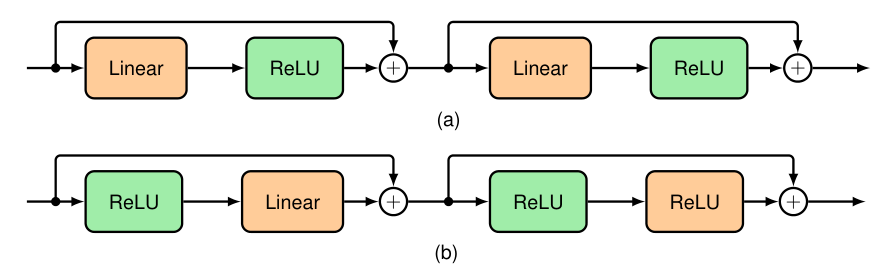
\includegraphics[width=0.5\textwidth]{figure-9-16.png}
        \caption{残差连接的两种放置方式。}
    \end{figure}
\end{frame}

% ============================================================
% 第五部分：总结
% ============================================================
\section{总结}

\begin{frame}
    \frametitle{5. 本节总结}
    \begin{itemize}
        \item \alert{深度网络训练困难}：
        \begin{itemize}
            \item 即使有批归一化，很多层的网络仍难以训练。
            \item \alert{破碎梯度}：极小的权重变化可导致梯度显著变化。
        \end{itemize}
        \item \alert{残差连接}：
        \begin{itemize}
            \item 将每个函数的输入加回输出：$\mathbf{z}_i = \mathbf{F}_i(\mathbf{z}_{i-1}) + \mathbf{z}_{i-1}$。
            \item \alert{残差块}：函数 + 残差连接。
            \item \alert{ResNet}：多个残差块串联。
            \item 函数学习恒等映射与期望输出之间的\alert{残差}。
        \end{itemize}
        \item \alert{效果}：
        \begin{itemize}
            \item 梯度对输入值\alert{更不敏感}。
            \item 创建\alert{更平滑的误差曲面}。
            \item 允许训练\alert{数百层}的极深网络。
            \item 整体函数由\alert{多个并行子网络}组成。
        \end{itemize}
        \item \alert{实现细节}：
        \begin{itemize}
            \item 维度匹配：可引入非方阵 $\mathbf{W}$。
            \item 残差连接位置：版本 (b)（ReLU 之后）更常用。
        \end{itemize}
    \end{itemize}
\end{frame}

% ============================================================
% 第六部分：参考文献
% ============================================================
\section{参考文献}

\begin{frame}
    \frametitle{6. 参考文献}
    \begin{itemize}
        \item 教材：Bishop, C. M. \& Bishop, H. (2023). Deep Learning Foundations and Concepts. Springer Nature Switzerland AG.
        \item He, K. et al. (2015). Deep residual learning for image recognition.
        \item Balduzzi, D. et al. (2017). The shattered gradients problem: If resnets are the answer, then what is the question?
        \item Li, H. et al. (2017). Visualizing the loss landscape of neural nets.
    \end{itemize}
\end{frame}

\end{document}